\documentclass[10pt,a4paper]{article}
\usepackage[margin=0.7in]{geometry}
\usepackage{booktabs}
\usepackage{array}
\usepackage{amsmath}
\usepackage{amssymb}
\usepackage{graphicx}
\usepackage{siunitx}
\usepackage{caption}
\usepackage{subcaption}
\usepackage[hidelinks]{hyperref}
\usepackage{xcolor}
\usepackage{pgfplots}
\pgfplotsset{compat=1.18}
\usepackage{enumitem}
\usepackage{listings}
\setlist[itemize]{leftmargin=*,itemsep=0pt,topsep=1pt,parsep=0pt}
\setlist[enumerate]{leftmargin=*,itemsep=0pt,topsep=1pt,parsep=0pt}
\setlength{\parskip}{1.5pt}
\setlength{\parindent}{0pt}
\captionsetup{font=small,skip=2pt}
\captionsetup[subfigure]{skip=0pt}
\renewcommand{\arraystretch}{1.02}
\lstset{basicstyle=\ttfamily\scriptsize,columns=fullflexible,aboveskip=1pt,belowskip=1pt,
        showstringspaces=false,keepspaces=true,breaklines=true,xleftmargin=1em,
        commentstyle=\color{gray!80!black}\itshape}

\title{\vspace{-3em}ASPP Coursework 2: Multi-GPU CUDA Wave Equation Solver}
\author{Exam No.\ B\texttt{281684}}
\date{\vspace{-0.3em}}

\begin{document}
\maketitle
\vspace{-1.0em}

\textbf{Notation.} SU/s $=$ site updates per second (product of lattice sites and time-steps per wall-clock second). $n_p$ $=$ number of MPI ranks, also the GPU count in this coursework (one rank per GPU). Throughout, the $z$ axis is the innermost (contiguous) storage dimension.

%==============================================================================
\section{Design and process}
\label{sec:design}

\paragraph{Why CUDA, and why two streams.}
CUDA gives direct control over the two resources that dominate this problem: the launch grid maps 1:1 onto a 3-D index space (no implicit compiler heuristic hides the memory traffic, which matters because the kernel is bandwidth-bound, see~\S\ref{par:roof}) and streams + events let us express the exact dependency graph between interior compute, halo pack, MPI, and boundary compute. We use \emph{two} streams because a rank has exactly two executors (one GPU, one CPU): one stream serialises pack and interior, erasing the only overlap opportunity; a third stream would split a chain that has no independent work to place on it.

\paragraph{Exact FLOP count.}
\label{par:flop}
Counted directly from \texttt{step\_kernel\_interior} and \texttt{damped\_update} in \texttt{wave\_cuda.cu}:

\begin{center}\small
\begin{tabular}{@{}lrrrrr@{}}
\toprule
Expression & adds & subs & muls & divs & total \\
\midrule
Laplacian $\sum_{6\text{ nbr}}u - 6u_c$              & 5 & 1 & 1 & 0 & 7 \\
$v = \text{factor}\cdot c_s^2 \cdot \Delta$          & 0 & 0 & 2 & 0 & 2 \\
Undamped tail $2u_c - u_{\text{prev}} + v$           & 1 & 1 & 1 & 0 & 3 \\
\midrule
\textbf{Interior (undamped) total}                   & 6 & 2 & 4 & 0 & \textbf{12} \\
\midrule
$\mathit{inv}{=}1/(1{+}d\Delta t)$; $n{=}1{-}d\Delta t$; $v\mathrel{*}{=}\mathit{inv}$ & 1 & 1 & 3 & 1 & 6 \\
$2\mathit{inv}\,u_c - n\,\mathit{inv}\,u_{\text{prev}} + v$ & 1 & 1 & 4 & 0 & 6 \\
\midrule
\textbf{Boundary (damped) total} ($7{+}2{+}12$)      & 7 & 3 & 10 & 1 & \textbf{21} \\
\bottomrule
\end{tabular}
\end{center}

Damping is only non-zero on the $x$ and $y$ boundary planes, so interior sites dominate and amortised FLOPs/site approach 12 as $L{\to}\infty$ (the $\mathcal{O}(L^{-1})$ boundary correction is below $0.1\%$ at $L\!\geq\!1000$). The rest of this report uses \textbf{12 FLOPs/site}.

\paragraph{Roofline: both bounds.}
\label{par:roof}
With 12 FLOPs/site, arithmetic intensities are $I_{\text{opt}}{=}0.30$ FLOP/B (optimistic 40 B/site: 4 unique reads + 1 write with L2 reuse) and $I_{\text{naive}}{=}0.14$ (88 B/site, 10 reads + 1 write). Device ridges $I_{\text{ridge}}{=}P_{\text{FP64}}/B_{\text{HBM}}$ are 4.8 (A100) and 10.0 (H100), far above our $I$. Translated into site throughput:

\begin{center}
\begin{tabular}{@{}lrr@{}}
\toprule
Ceiling & A100 (SU/s) & H100 (SU/s) \\
\midrule
Compute bound $P_{\text{FP64}}/12$                  & $8.08\!\times\!10^{11}$ & $2.79\!\times\!10^{12}$ \\
Bandwidth bound optimistic $B_{\text{HBM}}/40$      & $5.10\!\times\!10^{10}$ & $8.38\!\times\!10^{10}$ \\
Bandwidth bound naive $B_{\text{HBM}}/88$           & $2.32\!\times\!10^{10}$ & $3.81\!\times\!10^{10}$ \\
Our best single-GPU (Table~\ref{tab:roof})          & $3.56\!\times\!10^{10}$ & $7.68\!\times\!10^{10}$ \\
\bottomrule
\end{tabular}
\end{center}

We reach 4.4\% of the compute bound on A100 and 2.8\% on H100, but 70\% and 92\% of the optimistic bandwidth bound: the problem is unambiguously bandwidth-bound, and optimisation effort targets bytes-per-site.



\paragraph{Interior kernel and block shape.} 
The 32-wide $z$ dimension is exactly one warp, making each neighbour load a coalesced 256~B line: coalescing is all-or-nothing for a memory-bound kernel. A \texttt{(64,2,4)} block, by contrast, spans two warps requesting \emph{the same} $x$-plane and doubles in-flight L2 requests, costing $\approx 6\%$ on A100 in the \texttt{AWAVE\_CUDA\_BLOCK} sweep; \texttt{(32,8,2)} exceeds the register budget and regresses $\approx 1\%$. The depth-4 $x$ axis empirically gave the best balance between neighbour-plane reuse and occupancy across both GPUs: on H100 the effective traffic is close to half the naive 88~B/site model (Table~\ref{tab:roof}); A100 shows a smaller reduction.
\begin{lstlisting}[language=C++]
// grid = ceil(nz/32) x ceil(ny/4) x ceil(nx/4);   block = (32, 4, 4)
k = blockIdx.x*32 + threadIdx.x + 1;     // z direction; contiguous / fastest-varying
j = blockIdx.y*4  + threadIdx.y + 1;
i = blockIdx.z*4  + threadIdx.z + 1;     // outermost, strided
center = u_now[(i+1)*sx + (j+1)*sy + (k+1)];
lap    = sum_6_neighbours - 6*center;            // 7 FLOPs
value  = factor * cs2[c_idx] * lap;              // 2 FLOPs
u_next[...] = (d==0) ? 2*center - u_prev[...] + value   // 3 FLOPs
                     : damped_update(...);              // 12 FLOPs
\end{lstlisting}

\paragraph{Boundary-split kernels.}
Four kernels (one interior, three face) launch over \emph{disjoint} thread sets. Gains: $+4.51\%$ (A100) and $+22.18\%$ (H100) at $n_p{=}2$. The asymmetry is the evidence: H100's faster SMs issue at a rate where a warp that only evaluates the boundary predicate and early-returns still costs meaningful issue slots; A100, with slower issue, hides that idle time behind other latency. Splitting removes the wasted warps.

\paragraph{Why we did \emph{not} try to fix Z-face coalescing.}
A natural follow-up question is why we did not special-case the Z-perpendicular boundary face, where the $X\!-\!Y$ plane is stored with stride $n_z{+}2$ and so is not coalesced. The pack, unpack and \texttt{step\_kernel\_boundary\_z\_faces} kernels therefore do relatively inefficient DRAM access on that face. We deliberately did not tune it: the boundary work is $\mathcal{O}(L^2)$ while the interior is $\mathcal{O}(L^3)$, and the Z-face stage runs on \texttt{halo\_stream} concurrently with or immediately after the interior kernel on \texttt{compute\_stream}. The extra Z-face latency never enters the critical path of a step at the sizes of interest. Introducing a shared-memory transpose or a dedicated coalescing path would add tens of lines of code and complicate the overlap reasoning without reducing the step time. This is an instance of avoiding optimisation off the critical path.




\paragraph{Eight-phase step body.}
Phases (2) and (3) overlap: pack reads only boundary rows of \texttt{d\_now}; interior reads only strict interior; the two regions are disjoint so no CUDA sync is needed between streams during a step. Cross-stream events in (8) are device-side at zero CPU cost. The only host-side block is (5); by then the interior kernel is typically already done: on H100 $n_p{=}4$ at $1000^3$ the interior kernel takes about 3.5~ms, while a single \texttt{MPI\_Waitall} averages around 1.3~ms, and even two such waits per step remain below the interior time.
\begin{lstlisting}
for each step:
  (1) MPI_Irecv on active faces                    # host, no GPU dep
  (2) halo_stream:  pack_face_{x,y,z}<<<...>>>     # reads boundary rows
  (3) compute_stream: step_kernel_interior<<<...>>># disjoint from (2)
  (4) wait pack_done event; MPI_Isend(device ptr)
  (5) MPI_Waitall
  (6) halo_stream: unpack_face_{x,y,z}<<<...>>>
  (7) halo_stream: step_kernel_boundary_{x,y,z}_faces<<<...>>>
  (8) cudaStreamWaitEvent: next-step pack  waits for this interior;
                           next-step interior waits for this boundary
\end{lstlisting}

From a CPU/GPU coordination viewpoint, within a step the CPU side only issues light work (posting non-blocking MPI requests and recording/waiting on CUDA events), while the GPU runs the two independent streams in parallel. The CPU blocks exactly once per step, on \texttt{MPI\_Waitall}, and can do so without stalling the GPU because the compute stream has been fed all of its launches up front. In the common regime where interior time exceeds halo time, this structure means the GPU is continuously busy and the CPU is idle for most of each step.

\paragraph{Rejected optimisations.}
Every switch with a non-positive mean effect (Appendix~\ref{app:ab}) was removed from the hot code path. \emph{Shared-memory tiling} lost $2.3\!-\!4.6\%$: the working set already lives in L2 on both GPUs, so the extra load, \texttt{\_\_syncthreads} and re-read only add latency. \emph{Branchless damping} lost $\approx 0.1\%$ because the interior branch is warp-uniform ($d{=}0$) and costs nearly nothing; replacing it with an always-executed divide is strictly worse. \emph{Z-padding to 128~B} cost $\approx 0.4\%$: L2 absorbs mis-alignment but padding inflates total DRAM traffic. The \emph{\texttt{ob1}} OpenMPI stack regressed 41\% on H100 (loses CUDA IPC). \emph{CUDA Graphs} were also considered and dropped for single-node: their $\approx 10\,\mu$s launch saving is dwarfed by our $1\!-\!2$~ms interior kernel at $1000^3$; they become attractive at small per-rank problems on many-node runs (\S\ref{sec:further}). The final code defaults to the best-performing path while retaining a small number of robustness/tuning controls (notably MPI transfer mode and prewarm-iteration count) for portability.

\paragraph{Measurement conventions.}\mbox{}\par\nobreak\vspace{1pt}
\begin{center}\small
\begin{tabular}{@{}l p{0.85\linewidth}@{}}
\toprule
Timing       & \texttt{-nsteps 20}, \texttt{-io 0}, no restart, \texttt{-skip\_cpu 1} for timing only; 3 repeats, first sample discarded, best steady-state reported. \\
Correctness  & separate runs with CPU reference enabled, \texttt{ndiff=0} required before timing. \\
MPI layout   & most symmetric decomposition at each $n_p$ ($2{\times}2{\times}2$ at 8, $1{\times}2{\times}2$ at 4, $1{\times}1{\times}2$ at 2). \\
Build        & \texttt{-DCMAKE\_BUILD\_TYPE=Release -DAWAVE\_MODE=CUDA}, CUDA 13.0, mainline results use OpenMPI 4.1.9a1 with UCX-enabled CUDA-aware MPI (\texttt{hcoll}/\texttt{ucc} disabled). \\
\bottomrule
\end{tabular}
\end{center}

%==============================================================================
\section{Results}
\label{sec:results}

\paragraph{Environment and largest measurement.}
Per-GPU hardware: \texttt{A100-SXM4-80GB} / \texttt{H100-80GB-HBM3}; HBM peak $2.04$ / $3.35$~TB\,s$^{-1}$; L2 40 / 50~MB; FP64 non-sparse $9.7$ / $33.5$~TFLOP\,s$^{-1}$; NVLink $600$ / $900$~GB\,s$^{-1}$ bidirectional~\cite{a100ds,h100ds}. All reported mainline performance points were obtained only after a separate correctness run with the CPU reference enabled (\texttt{ndiff=0}). The largest device-path measurement we obtained was \textbf{H100 $n_p{=}8$ at $2500^3$} ($1.56\!\times\!10^{10}$ sites; $4.12\!\times\!10^{11}$ SU/s; this point is \emph{reference only}). The unmodified submission cannot accommodate $2500^3$ on a single EIDF node because the driver allocates both CPU and GPU mirror states ($\approx 96$\,B per host point across six arrays times two mirrors, giving $\approx 1.5$~TB at $2500^3 \times 8$). For this one point we removed the CPU-mirror allocation from \texttt{main.cpp} (valid under \texttt{-skip\_cpu}) and reconstructed the initial condition on-device in \texttt{wave\_cuda.cu}; GPU kernels and MPI path are unchanged, so the measurement reflects device-path performance even though the exact workflow is not reproducible from the submitted sources. Details in Appendix~\ref{app:2500}. A100 $n_p{=}8$ for sizes $\geq\!1500$ could not be scheduled within the coursework window and is marked N/A.

\paragraph{Single-GPU roofline validation.}
Inverting measured throughput $S$ to effective traffic $B_{\text{eff}}{=}B_{\text{HBM}}/S$ gives Table~\ref{tab:roof}. H100 sits at $40.6\!-\!43.7$~B/site, close to the optimistic bound, consistent with substantial L2 reuse that removes most of the other $\approx\!48$~B/site in the naive model. A100 lands $\approx\!58$~B/site: its smaller 40~MB L2 offers less headroom for the same block shape, so neighbour-plane reuse is less complete.

\begin{table}[h]
\centering\small
\caption{Single-GPU roofline validation at $n_p{=}1$. \%-ages are vs the HBM peak at 40~B/site optimistic bound, the 88~B/site naive bound, and $P_{\text{FP64}}/12$ compute bound.}
\label{tab:roof}
\begin{tabular}{@{}lrrrrr@{}}
\toprule
GPU / size & SU/s & $B_{\text{eff}}$ (B/site) & \% of BW opt & \% of BW naive & \% of compute \\
\midrule
H100 / $256^3$  & $8.26\!\times\!10^{10}$ & 40.6 & $\mathbf{98.6\%}$ & $217\%$ & $3.0\%$ \\
H100 / $512^3$  & $7.67\!\times\!10^{10}$ & 43.7 & $91.6\%$          & $201\%$ & $2.7\%$ \\
H100 / $1000^3$ & $7.68\!\times\!10^{10}$ & 43.6 & $91.7\%$          & $202\%$ & $2.8\%$ \\
A100 / $256^3$  & $3.46\!\times\!10^{10}$ & 59.0 & $67.8\%$          & $149\%$ & $4.3\%$ \\
A100 / $512^3$  & $3.44\!\times\!10^{10}$ & 59.3 & $67.4\%$          & $148\%$ & $4.3\%$ \\
A100 / $1000^3$ & $3.56\!\times\!10^{10}$ & 57.3 & $69.8\%$          & $154\%$ & $4.4\%$ \\
\bottomrule
\end{tabular}
\end{table}

H100 exceeding the naive bound is consistent with substantial L2 reuse: the kernel appears to see less DRAM traffic than a 10-reads-1-write model predicts.

\begin{figure}[h]
\centering
\begin{subfigure}{0.48\linewidth}
\centering
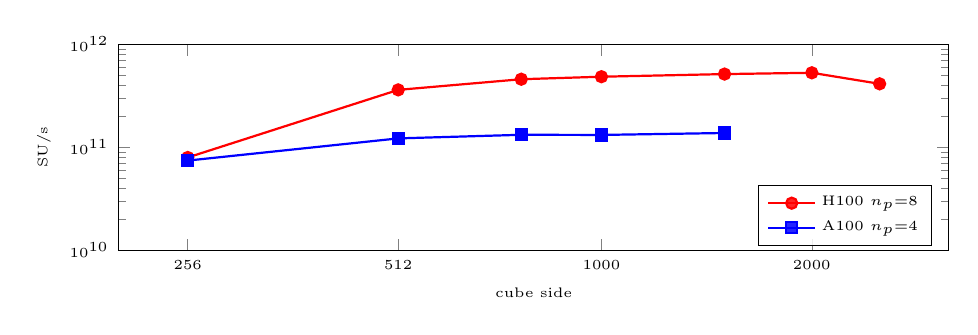
\begin{tikzpicture}
\begin{axis}[width=\linewidth,height=4.2cm,xlabel={cube side},ylabel={SU/s},
    xmode=log,log basis x=2,ymode=log,ymin=1e10,ymax=1e12,
    xtick={256,512,1000,2000},xticklabels={256,512,1000,2000},
    legend style={font=\tiny,at={(0.98,0.02)},anchor=south east,
                  fill=white,fill opacity=0.85,draw opacity=1,text opacity=1},
    tick label style={font=\tiny},label style={font=\tiny}]
\addplot[mark=*,color=red,thick] coordinates
  {(256,7.954e10)(512,3.600e11)(768,4.567e11)(1000,4.830e11)(1500,5.123e11)(2000,5.273e11)(2500,4.121e11)};
\addlegendentry{H100 $n_p{=}8$}
\addplot[mark=square*,color=blue,thick] coordinates
  {(256,7.421e10)(512,1.218e11)(768,1.320e11)(1000,1.316e11)(1500,1.374e11)};
\addlegendentry{A100 $n_p{=}4$}
\end{axis}
\end{tikzpicture}
\caption{Throughput vs cube side (log$_2$ / log).}
\label{fig:size}
\end{subfigure}\hfill
\begin{subfigure}{0.48\linewidth}
\centering
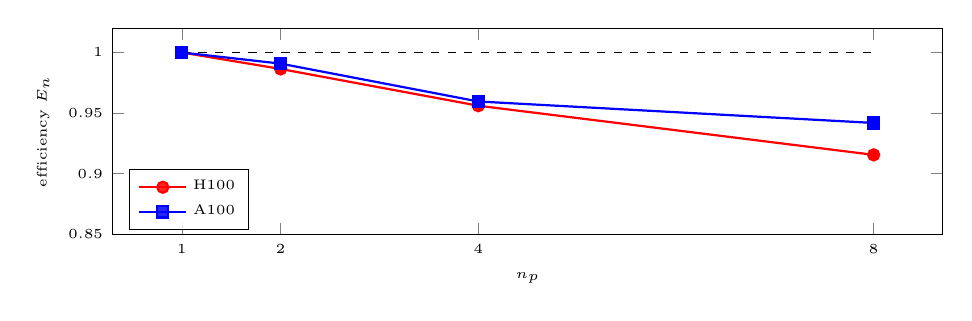
\begin{tikzpicture}
\begin{axis}[width=\linewidth,height=4.2cm,xlabel={$n_p$},ylabel={efficiency $E_n$},
    ymin=0.85,ymax=1.02,xtick={1,2,4,8},
    legend style={font=\tiny,at={(0.02,0.02)},anchor=south west,
                  fill=white,fill opacity=0.85,draw opacity=1,text opacity=1},
    tick label style={font=\tiny},label style={font=\tiny}]
\addplot[mark=*,color=red,thick] coordinates
  {(1,1.0)(2,0.9864)(4,0.9561)(8,0.9156)};
\addlegendentry{H100}
\addplot[mark=square*,color=blue,thick] coordinates
  {(1,1.0)(2,0.9908)(4,0.9596)(8,0.9419)};
\addlegendentry{A100}
\addplot[color=black,dashed,thin,domain=1:8] {1};
\end{axis}
\end{tikzpicture}
\caption{Strong-scaling efficiency at $1000^3$.}
\label{fig:eff}
\end{subfigure}
\caption{(a) Throughput across problem sizes; A100 $n_p{=}8$ is omitted from the main curve because its large-size coverage is incomplete and its small-size points fall in a kernel-too-small regime (see text). (b) Strong scaling at $1000^3$.}
\label{fig:main}
\end{figure}

\paragraph{Strong scaling at $1000^3$.}
Efficiency $E_n{=}S_n/(n S_1)$ (Table~\ref{tab:scale}, Figure~\ref{fig:eff}): H100 holds $91.6\%$ at $n_p{=}8$; A100 holds $94.2\%$. The one anomalous point is H100 $n_p{=}8$ at $256^3$ in Figure~\ref{fig:size}: each rank owns only a very small subdomain, so launch and MPI overhead become comparable to the useful compute payload. This is a kernel-too-small regime rather than evidence of a correctness problem, and the behaviour largely disappears by $512^3$. A100 $n_p{=}8$ large-size coverage is incomplete and data-consistency is not fully confirmed, so it is not drawn as a main curve in Figure~\ref{fig:size}; the small-size points we did capture live in the same kernel-too-small regime. The dip at $2500^3$ in the H100 $n_p{=}8$ curve is consistent with weaker cache reuse and a less favourable memory regime at that size; however, this point also required the special timing path described above and is interpreted cautiously.

\begin{table}[h]
\centering\small
\caption{Strong scaling at $1000^3$. Extra overhead $=1-E_n$.}
\label{tab:scale}
\begin{tabular}{@{}rrrrrr@{}}
\toprule
$n_p$ & A100 SU/s & $E_n$ & H100 SU/s & $E_n$ & H100 extra overhead \\
\midrule
1 & $3.514\!\times\!10^{10}$ & $100.0\%$ & $6.669\!\times\!10^{10}$ & $100.0\%$ & $0.0\%$ \\
2 & $6.963\!\times\!10^{10}$ & $99.1\%$  & $1.316\!\times\!10^{11}$ & $98.6\%$  & $1.4\%$ \\
4 & $1.349\!\times\!10^{11}$ & $96.0\%$  & $2.551\!\times\!10^{11}$ & $95.6\%$  & $4.4\%$ \\
8 & $2.648\!\times\!10^{11}$ & $94.2\%$  & $4.885\!\times\!10^{11}$ & $91.6\%$  & $8.4\%$ \\
\bottomrule
\end{tabular}
\end{table}

\paragraph{Weak scaling (discussion) and communication.}
A dedicated weak-scaling sweep was not feasible. The $1000^3$ strong-scaling series does not replace weak scaling, but it provides a useful communication anchor: as the per-rank subdomain shrinks, the additional scaling loss remains modest ($8.4\%$ on H100 and $5.8\%$ on A100 at $n_p{=}8$). NSYS traces (Appendix~\ref{app:nsys}) report \texttt{MPI\_Waitall} average call durations of $1.3\!-\!2.9$~ms on H100 $n_p{=}4/8$. With two \texttt{MPI\_Waitall} calls per step (one on the receive set, one on the send set), per-step wait totals $\approx\!2.6\!-\!5.8$~ms while interior time is only $3.5$/$1.75$~ms; on H100 $n_p{=}4$ the wait-fraction metric reads $40.4\%$ yet $E_4{=}95.6\%$. This gap, which plausibly reflects the dual-stream pipeline hiding most waits behind interior compute, collapses at $n_p{=}8$ where per-step wait exceeds interior time and $E_8$ falls to $91.6\%$.

\paragraph{Decomposition and surface-to-volume.}
At every GPU count we used the most symmetric decomposition available to minimise the surface-to-volume ratio and hence communication volume per step. At $n_p{=}8$ we also measured two asymmetric alternatives: $1{\times}2{\times}4$ lost $\approx\!5\%$ and $1{\times}1{\times}8$ lost $\approx\!14\%$ at $1000^3$ relative to $2{\times}2{\times}2$, matching the predicted face-area ratios ($1{\times}1{\times}8$ has $\approx\!2.3\times$ the face area of the cube). This validates the symmetric-decomposition rule in our measurement conventions.

%==============================================================================
\section{Further work: scaling to many nodes}
\label{sec:further}

\paragraph{Intra-node vs inter-node.}
Intra-node halos cross NVLink at $600\!-\!900$~GB/s with $\sim\!\mu$s latency. Across nodes, traffic follows PCIe\,$\to$\,NIC\,$\to$\,IB\,$\to$\,NIC\,$\to$\,PCIe at typically 25~GB/s per NDR-200 link with $\mathcal{O}(1\!-\!2\,\mu$s) latency plus software stack overhead. At the measured anchor (total problem $1000^3$, $n_p{=}8$, $2{\times}2{\times}2$ decomposition) each rank owns a $500^3$ subdomain and one face is $500^2{\times}8\,\text{B}{\approx}\,2$~MB: transferring one face takes $\sim\!3\,\mu$s over NVLink, $\sim\!80\,\mu$s over IB. Against a measured H100 $n_p{=}8$ interior of $1.75$~ms, a $30\times$ slower fabric still fits under the overlap ceiling, but the margin collapses.

A simple per-step model captures this: $T_{\text{step}} \approx \max(T_{\text{int}}, T_{\text{halo}}) + \epsilon_{\text{latency}}$, where $T_{\text{halo}} \approx V_{\text{face}}/B_{\text{fabric}} + L_{\text{fabric}}$ and $V_{\text{face}}$ is the per-face halo volume. At this anchor, $T_{\text{int}} \gg T_{\text{halo}}$ intra-node, so the pipeline hides communication; as the effective fabric bandwidth drops, the crossover $T_{\text{halo}}{=}T_{\text{int}}$ determines the onset of visible efficiency loss. (This is an optimistic single-face model and ignores multi-face contention and imperfect overlap.)

\paragraph{Indicative efficiency forecasts (order-of-magnitude).}
Using Appendix~\ref{app:nsys} only as a coarse anchor, we infer that the exposed communication fraction is small on H100 $n_p{=}2$ and grows materially by $n_p{=}8$ as exposed communication time becomes comparable $T_{\text{int}}$. Extrapolating the same $T_{\text{halo}}/T_{\text{int}}$ ratio to a $2{\times}2{\times}2$-per-node layout of H100s at $1000^3$/GPU:
\begin{itemize}
\item 2\,--\,4 nodes: about $80\!-\!85\%$ efficiency. Only one Cartesian axis becomes inter-node in the smallest multi-node layouts.
\item 16\,--\,64 nodes: roughly $60\!-\!70\%$. IB saturates at $\sim\!20$~GB/s per link, so $T_{\text{halo}}{\sim}T_{\text{int}}$.
\item 100$+$ nodes ($>\!800$ GPUs): at most $\sim\!40\%$ unless per-rank problem grows; latency dominates and any global reductions pile on.
\end{itemize}
These percentages are indicative rather than model-derived predictions; they report the $T_{\text{halo}}/T_{\text{int}}$ ratios implied by the bandwidth / latency figures above as an order-of-magnitude guide only.

\paragraph{Code changes to reach that scale.}
\textbf{(i)~Persistent MPI requests} (\texttt{MPI\_Send\_init}/\texttt{Start}) remove request-object construction from the hot loop. \textbf{(ii)~CUDA Graphs} capture the 8-phase body once and replay; the $\approx\!10\,\mu$s launch saving compounds on small per-rank problems. This is the optimisation we rejected for single-node and would adopt here. \textbf{(iii)~Temporal blocking}: sweep $K$ steps before exchanging halos deepened by $K$. $B_{\text{eff}}$ drops to $\sim\!48/K$ and halo volume grows by $K\times$ per exchange but is amortised over $K$ steps, so net communication pressure drops $\sim\!K\times$. For $K{=}4$ this could materially improve many-node scalability, at the cost of a $K$-deep ghost region and careful handling of the time-dependent boundary damping. \textbf{(iv)~Topology-aware placement} via \texttt{MPI\_Dist\_graph\_create\_adjacent} on the 3-D Cartesian neighbour graph so the neighbouring Cartesian ranks are mapped to nearby network locations. \textbf{(v)~NCCL or tree-reduction} for any future global reductions.

\paragraph{Beyond the solver.}
At $\mathcal{O}(1000)$ GPUs the CPU reference path no longer fits in one node of host RAM, so correctness would move to computed invariants (energy, analytic Gaussian-pulse solution). Checkpoint frequency must become adaptive. IO is out of scope by brief; in production it would be the next limit.

%==============================================================================
\clearpage
\appendix
\section{Optimisation A/B table}
\label{app:ab}
Each row aggregates 3\,--\,5 repeat runs. $\Delta$ is the mean percentage change of best-steady-state SU/s against the control. 

\begin{center}\small
\begin{tabular}{@{}lllrrc@{}}
\toprule
Switch & Rationale & Measured at & A100 $\Delta$ & H100 $\Delta$ & Decision \\
\midrule
Boundary-split kernels & remove interior early-return & $n_p{=}2$ & $+4.51\%$ & $+22.18\%$ & adopted \\
Block shape $(32,4,4)$ & warp-coalesced $k$ + L2 $x$-reuse & $n_p{=}1$ & $+6.03\%$ & $+0.04\%$ & adopted (default) \\
Shared-memory tiling & reduce global reads & $n_p{=}1$ & $-2.32\%$ & $-4.59\%$ & rejected \\
MPI mode host vs device & CUDA-aware vs staging & $n_p{=}2$ & host $-10.13\%$ & host $-3.23\%$ & adopted \texttt{device} \\
OpenMPI \texttt{ob1} stack & alternative BTL & $n_p{=}2$ & $-0.08\%$ & $-41.45\%$ & rejected \\
\texttt{MPI\_Waitsome} loop & earlier unpack & $n_p{=}2$ & $-0.03\%$ & $-0.56\%$ & rejected \\
Damping branchless & avoid warp divergence & $n_p{=}1$ & $-0.09\%$ & $\approx 0$ & rejected \\
$z$-padding (128~B align) & coalesce alignment & $n_p{=}1$ & $-0.37\%$ & $-0.51\%$ & rejected \\
\bottomrule
\end{tabular}
\end{center}

\section{Nsight Systems communication table}
\label{app:nsys}
Totals over 20 profiled steps at $1000^3$. Wait-fraction $=T_{\text{wait,tot}}/(T_{\text{int,tot}}{+}T_{\text{wait,tot}})$; overlap proxy $=\max(0,1-T_{\text{wait,tot}}/T_{\text{int,tot}})$.

\begin{center}\small
\begin{tabular}{@{}llrrrrr@{}}
\toprule
GPU & $n_p$ & interior (ms) & Waitall avg (ms) & Waitall tot (ms) & wait frac. & overlap proxy \\
\midrule
A100 & 2 & 13.56 & 0.24 & 9.68    & $3.2\%$  & $96.4\%$ \\
A100 & 4 & 6.77  & 0.56 & 45.07   & $13.3\%$ & $83.4\%$ \\
H100 & 2 & 7.17  & 0.47 & 18.81   & $10.9\%$ & $86.9\%$ \\
H100 & 4 & 3.51  & 1.28 & 102.55  & $40.4\%$ & $27.0\%$ \\
H100 & 8 & 1.75  & 2.89 & 462.28  & $75.3\%$ & $0.0\%$  \\
\bottomrule
\end{tabular}
\end{center}
Wait-fraction is a wall-clock waiting-behaviour metric rather than a true communication-cost share: on H100 $n_p{=}4$ it reads $40.4\%$ while strong-scaling loss is only $4.4\%$, because much of the wait occurs while the interior kernel is still executing on \texttt{compute\_stream}. (Note: \texttt{Waitall tot} values at larger $n_p$ reflect Nsight Systems aggregating metrics across multiple profiled ranks, scaling the total call count beyond a single rank's 40 calls; the derived \texttt{wait frac} and \texttt{avg} columns remain mathematically representative. Interpret \texttt{avg} as the mean duration of a single \texttt{MPI\_Waitall} call, not a per-step wait; each step issues two such calls.)

\section{Note on the $2500^3$ reference measurement}
\label{app:2500}
The unmodified driver stores two mirrored host simulations (CPU reference + CUDA state), across six \texttt{double} arrays (\texttt{u\_prev},\texttt{u\_now},\texttt{u\_next},\texttt{cs2},\texttt{damp},\texttt{sos}) $\approx 96$~B per lattice point. At $2500^3$ spread over 8 ranks on one node, this totals roughly 1.5~TB of host memory, exceeding the 512~GB per-node RAM.

For the $2500^3$ reference point only, we made two targeted adjustments (not part of the submitted source):
\begin{itemize}
\item \texttt{main.cpp}: under \texttt{-skip\_cpu 1}, skip the CPU-mirror allocation and clone path.
\item \texttt{wave\_cuda.cu}: a small initialiser that reconstructs the initial condition directly on device from the same analytic parameters, removing the dependence on a host copy. This runs once before the time loop and does not affect per-step timing.
\end{itemize}
GPU kernels and MPI path are unchanged from the submission. The measurement reflects device-path performance; we report it as a reference only, and clearly label it in Figure~\ref{fig:size} and the surrounding text.

\begin{thebibliography}{10}\small
\bibitem{a100ds} NVIDIA Corporation. \emph{NVIDIA A100 Tensor Core GPU Architecture}. White paper, 2020. \url{https://images.nvidia.com/aem-dam/en-zz/Solutions/data-center/nvidia-ampere-architecture-whitepaper.pdf}
\bibitem{h100ds} NVIDIA Corporation. \emph{NVIDIA H100 Tensor Core GPU Architecture}. White paper, 2022. \url{https://resources.nvidia.com/en-us-tensor-core/gtc22-whitepaper-hopper}
\bibitem{roofline} S.~Williams, A.~Waterman, and D.~Patterson. Roofline: An Insightful Visual Performance Model for Multicore Architectures. \emph{Communications of the ACM}, 52(4):65--76, 2009. \url{https://doi.org/10.1145/1498765.1498785}
\bibitem{ompi} Open MPI Project. \emph{Open MPI v4.1.x documentation}. \url{https://docs.open-mpi.org/en/v4.1.x/}
\bibitem{nsys} NVIDIA Corporation. \emph{Nsight Systems User Guide}. \url{https://docs.nvidia.com/nsight-systems/UserGuide/}
\end{thebibliography}

\end{document}
